\documentclass[10 pt]{article}

\usepackage[top= 30mm, bottom=30mm, left=35mm, right=35mm]{geometry}
\usepackage[OT2]{fontenc}
\usepackage[serbian]{babel}
\usepackage{hyperref}
\usepackage{graphicx}
\usepackage{float}
\usepackage{caption}

\hypersetup{
    colorlinks=true,
    linktoc=all,
    linkcolor=blue,
}

\begin{document}
	
\begin{titlepage} 
	\centering 
	
	\rule{\textwidth}{1pt}
	
	\vspace{2pt}\vspace{-\baselineskip} 
	
	\rule{\textwidth}{0.4pt}
	
	\vspace{0.025\textheight}

	{\Huge Baza podataka za Stomatoloshku ordinaciju}
	
	\vspace{0.020\textheight}
	
	\rule{0.5\textwidth}{1pt}
	
	\vspace{0.5\textheight}
	
	\begin{minipage}{0.4\textwidth}
		\begin{flushleft} \large
			\emph{Autor:}\\
			Marija Mijailovic1 1093/2017
		\end{flushleft}
	\end{minipage}
	~
	\begin{minipage}{0.4\textwidth}
		\begin{flushright} \large
			\emph{Asistent:} \\
			Ivana Tanasijevic1
		\end{flushright}
	\end{minipage}\\[2cm]

	{\large \today}\\[2cm]
	
	\rule{1\textwidth}{1.5pt}
	
\end{titlepage}
	

\thispagestyle{empty}

\newpage
\renewcommand*\contentsname{Sadrzhaj:}
\tableofcontents

\newpage
\section{Opis baze}

\textbf{Stomatoloshka ordinacija} chuva sledec1e informacije:
\begin{itemize} 
	\item Pacijent(idPacijent, Ime, Prezime, DatumRodjenja, Adresa, Telefon, DatumOtvaranjaKartona, UkupanDug, Plac1eno, Napomena),
	\item PochetnoStanje(idPochetnoStanje, Zub0-Zub31),
	\item Zaposlen(idZaposleni, Ime, Prezime), 
	\item Zub(idZub), 
	\item Bolest(idBolest, OpisBolesti),
	\item Stolica(idOprema, BrojStolice), 
	\item Intervenca(idIntervencija, Datum) 
	\item SpisakIntervencija(idSpisak, NazivIntervencije, Cena),
	\item OblastIntervencije(idOblast, NazivOblasti)
\end{itemize}
Zaposlen u ordinaciji mozhe biti Tehnichar ili Stomatolog, za Stomatologa se chuva josh i informacija o statusu zaposlenja. Pacijent je osoba koja dolazi u ordinaciju radi obavljanja intervencije, za svakog pacijenta se chuva informacija o pochetnom stanju svih zuba, sa kojim je doshao prvi put u ordinaciju. Nad jednim pacijentom se mozhe obaviti vishe intervencija, dok jedna intervencija odgovara jednom pacijentu. Stomatolog mozhe da izvrshi jednu ili vishe intervencija nad pacijentom. Dok tehnichar mozhe, ali i ne mora da izvrshi intervenciju nad pacijentom. Jedna intervencija se mozhe obaviti na vishe stolica, a na stolici mozhe biti obavljeno vishe intervencija,medjutim ne mora biti obavljena ni jedna. Spisak intervencija sadrzhi vishe intervencija, ali mora imati bar jednu. Svaka intervencija sa spiska intervencija pripada tachno jednoj oblasti intervencija. Nad jednim zubom mozhe biti izvrsheno vishe intervencija. Takodje svaki zub mozhe imati i jednu ili vishe bolesti. Dok bolest moze zahvatiti vishe zuba,ali ne mora ni jedan. Odgovarajuc1i dijagram dat je na slici \ref{fig:dijagram}
\\
\\
\textbf{Zadovoljenost uslova:}
\begin{itemize}
	\item Nezavisni entiteti: Zaposleni, Pacijent, Stolica, OblastIntervencije, Bolest
	\item Agregirani entiteti: Obavlja, Ima
	\item Zavisni entiteti: Intervencija, Pochetno stanje
	\item Trigeri: 
		\begin{itemize}
			\item Nakon obavljene intervencije azhurira se dug pacijenta prema ordinaciji.
			\item Promena cene intervencije vazhi od dana izmene.
		\end{itemize}	
\end{itemize}

\begin{figure}[H]
	\centering
	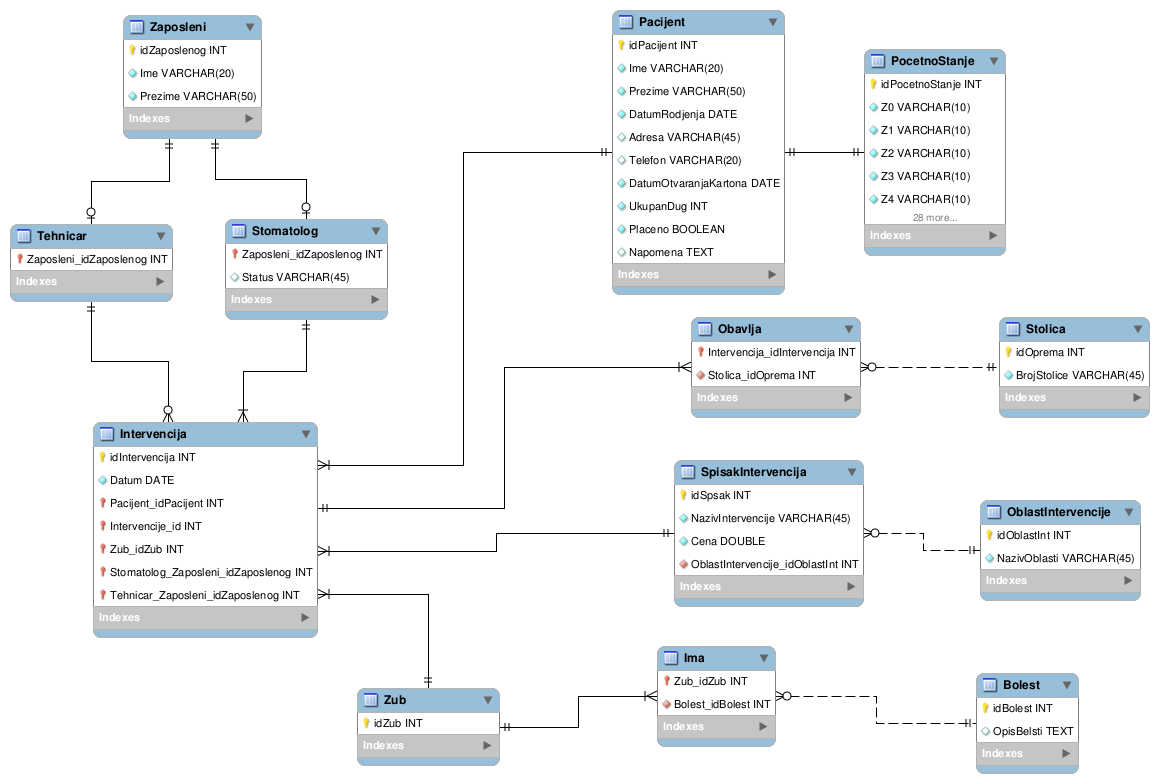
\includegraphics[width=15cm,height=15cm,keepaspectratio]{StomatoloskaOrdinacija.png}\\
	\caption{Stomatoloshka ordinacija \label{fig:dijagram}}
\end{figure}

\end{document} 